\documentclass{article}
\usepackage{microtype}
\usepackage{graphicx}
\usepackage{booktabs}
\usepackage{amsmath,amssymb}
\usepackage{hyperref}
\usepackage[accepted]{icml2027}

% Auto-generated macros from raw TensorBoard (.tfevents) & W&B logs via ./veriloop bind
% Auto-generated by VeriLoop paper_bind.py — DO NOT EDIT BY HAND
% Every macro traces verbatim to bound_metrics.txt
\newcommand{\vlCMLinearCalEce}{0.0236$\pm$0.0061}
\newcommand{\vlCMLinearCalEceMean}{0.0236}
\newcommand{\vlCMLinearCalEceCi}{[0.0084, 0.0388]}
\newcommand{\vlCMLinearCalNll}{1.8050$\pm$0.0130}
\newcommand{\vlCMLinearCalNllMean}{1.8050}
\newcommand{\vlCMLinearCalNllCi}{[1.7726, 1.8374]}
\newcommand{\vlCMLinearTempT}{1.4978$\pm$0.0529}
\newcommand{\vlCMLinearTempTMean}{1.4978}
\newcommand{\vlCMLinearTempTCi}{[1.3664, 1.6292]}
\newcommand{\vlCMLinearTestAcc}{0.3692$\pm$0.0090}
\newcommand{\vlCMLinearTestAccMean}{0.3692}
\newcommand{\vlCMLinearTestAccCi}{[0.3468, 0.3915]}
\newcommand{\vlCMLinearTestEce}{0.0959$\pm$0.0135}
\newcommand{\vlCMLinearTestEceMean}{0.0959}
\newcommand{\vlCMLinearTestEceCi}{[0.0624, 0.1293]}
\newcommand{\vlCMLinearTestNll}{1.8679$\pm$0.0210}
\newcommand{\vlCMLinearTestNllMean}{1.8679}
\newcommand{\vlCMLinearTestNllCi}{[1.8157, 1.9200]}
\newcommand{\vlCMLinearValAcc}{0.3722$\pm$0.0025}
\newcommand{\vlCMLinearValAccMean}{0.3722}
\newcommand{\vlCMLinearValAccCi}{[0.3660, 0.3784]}
\newcommand{\vlCMPlaincnnCalEce}{0.0127$\pm$0.0048}
\newcommand{\vlCMPlaincnnCalEceMean}{0.0127}
\newcommand{\vlCMPlaincnnCalEceCi}{[0.0009, 0.0246]}
\newcommand{\vlCMPlaincnnCalNll}{0.6407$\pm$0.0041}
\newcommand{\vlCMPlaincnnCalNllMean}{0.6407}
\newcommand{\vlCMPlaincnnCalNllCi}{[0.6305, 0.6509]}
\newcommand{\vlCMPlaincnnTempT}{1.1669$\pm$0.0468}
\newcommand{\vlCMPlaincnnTempTMean}{1.1669}
\newcommand{\vlCMPlaincnnTempTCi}{[1.0506, 1.2831]}
\newcommand{\vlCMPlaincnnTestAcc}{0.7787$\pm$0.0029}
\newcommand{\vlCMPlaincnnTestAccMean}{0.7787}
\newcommand{\vlCMPlaincnnTestAccCi}{[0.7715, 0.7860]}
\newcommand{\vlCMPlaincnnTestEce}{0.0281$\pm$0.0038}
\newcommand{\vlCMPlaincnnTestEceMean}{0.0281}
\newcommand{\vlCMPlaincnnTestEceCi}{[0.0186, 0.0376]}
\newcommand{\vlCMPlaincnnTestNll}{0.6484$\pm$0.0016}
\newcommand{\vlCMPlaincnnTestNllMean}{0.6484}
\newcommand{\vlCMPlaincnnTestNllCi}{[0.6443, 0.6525]}
\newcommand{\vlCMPlaincnnValAcc}{0.7838$\pm$0.0043}
\newcommand{\vlCMPlaincnnValAccMean}{0.7838}
\newcommand{\vlCMPlaincnnValAccCi}{[0.7732, 0.7944]}
\newcommand{\vlCMResnetBaseCalEce}{0.0098$\pm$0.0023}
\newcommand{\vlCMResnetBaseCalEceMean}{0.0098}
\newcommand{\vlCMResnetBaseCalEceCi}{[0.0040, 0.0156]}
\newcommand{\vlCMResnetBaseCalNll}{0.5624$\pm$0.0170}
\newcommand{\vlCMResnetBaseCalNllMean}{0.5624}
\newcommand{\vlCMResnetBaseCalNllCi}{[0.5202, 0.6046]}
\newcommand{\vlCMResnetBaseTempT}{2.6460$\pm$0.1037}
\newcommand{\vlCMResnetBaseTempTMean}{2.6460}
\newcommand{\vlCMResnetBaseTempTCi}{[2.3883, 2.9037]}
\newcommand{\vlCMResnetBaseTestAcc}{0.8112$\pm$0.0058}
\newcommand{\vlCMResnetBaseTestAccMean}{0.8112}
\newcommand{\vlCMResnetBaseTestAccCi}{[0.7967, 0.8257]}
\newcommand{\vlCMResnetBaseTestEce}{0.1261$\pm$0.0074}
\newcommand{\vlCMResnetBaseTestEceMean}{0.1261}
\newcommand{\vlCMResnetBaseTestEceCi}{[0.1078, 0.1444]}
\newcommand{\vlCMResnetBaseTestNll}{0.9155$\pm$0.0716}
\newcommand{\vlCMResnetBaseTestNllMean}{0.9155}
\newcommand{\vlCMResnetBaseTestNllCi}{[0.7375, 1.0935]}
\newcommand{\vlCMResnetBaseValAcc}{0.8134$\pm$0.0052}
\newcommand{\vlCMResnetBaseValAccMean}{0.8134}
\newcommand{\vlCMResnetBaseValAccCi}{[0.8005, 0.8263]}
\newcommand{\vlCMResnetAugCalEce}{0.0088$\pm$0.0006}
\newcommand{\vlCMResnetAugCalEceMean}{0.0088}
\newcommand{\vlCMResnetAugCalEceCi}{[0.0073, 0.0103]}
\newcommand{\vlCMResnetAugCalNll}{0.3641$\pm$0.0083}
\newcommand{\vlCMResnetAugCalNllMean}{0.3641}
\newcommand{\vlCMResnetAugCalNllCi}{[0.3435, 0.3847]}
\newcommand{\vlCMResnetAugTempT}{1.5584$\pm$0.0720}
\newcommand{\vlCMResnetAugTempTMean}{1.5584}
\newcommand{\vlCMResnetAugTempTCi}{[1.3794, 1.7373]}
\newcommand{\vlCMResnetAugTestAcc}{0.8764$\pm$0.0034}
\newcommand{\vlCMResnetAugTestAccMean}{0.8764}
\newcommand{\vlCMResnetAugTestAccCi}{[0.8679, 0.8850]}
\newcommand{\vlCMResnetAugTestEce}{0.0487$\pm$0.0047}
\newcommand{\vlCMResnetAugTestEceMean}{0.0487}
\newcommand{\vlCMResnetAugTestEceCi}{[0.0371, 0.0603]}
\newcommand{\vlCMResnetAugTestNll}{0.4112$\pm$0.0154}
\newcommand{\vlCMResnetAugTestNllMean}{0.4112}
\newcommand{\vlCMResnetAugTestNllCi}{[0.3731, 0.4494]}
\newcommand{\vlCMResnetAugValAcc}{0.8760$\pm$0.0075}
\newcommand{\vlCMResnetAugValAccMean}{0.8760}
\newcommand{\vlCMResnetAugValAccCi}{[0.8572, 0.8948]}
\newcommand{\vlCMResnetAugCosineCalEce}{0.0061$\pm$0.0015}
\newcommand{\vlCMResnetAugCosineCalEceMean}{0.0061}
\newcommand{\vlCMResnetAugCosineCalEceCi}{[0.0023, 0.0098]}
\newcommand{\vlCMResnetAugCosineCalNll}{0.2500$\pm$0.0031}
\newcommand{\vlCMResnetAugCosineCalNllMean}{0.2500}
\newcommand{\vlCMResnetAugCosineCalNllCi}{[0.2424, 0.2576]}
\newcommand{\vlCMResnetAugCosineTempT}{1.4338$\pm$0.0128}
\newcommand{\vlCMResnetAugCosineTempTMean}{1.4338}
\newcommand{\vlCMResnetAugCosineTempTCi}{[1.4021, 1.4655]}
\newcommand{\vlCMResnetAugCosineTestAcc}{0.9152$\pm$0.0011}
\newcommand{\vlCMResnetAugCosineTestAccMean}{0.9152}
\newcommand{\vlCMResnetAugCosineTestAccCi}{[0.9124, 0.9179]}
\newcommand{\vlCMResnetAugCosineTestEce}{0.0324$\pm$0.0013}
\newcommand{\vlCMResnetAugCosineTestEceMean}{0.0324}
\newcommand{\vlCMResnetAugCosineTestEceCi}{[0.0291, 0.0356]}
\newcommand{\vlCMResnetAugCosineTestNll}{0.2728$\pm$0.0038}
\newcommand{\vlCMResnetAugCosineTestNllMean}{0.2728}
\newcommand{\vlCMResnetAugCosineTestNllCi}{[0.2633, 0.2822]}
\newcommand{\vlCMResnetAugCosineValAcc}{0.9160$\pm$0.0024}
\newcommand{\vlCMResnetAugCosineValAccMean}{0.9160}
\newcommand{\vlCMResnetAugCosineValAccCi}{[0.9100, 0.9220]}
\newcommand{\vlCMResnetLsCalEce}{0.0116$\pm$0.0033}
\newcommand{\vlCMResnetLsCalEceMean}{0.0116}
\newcommand{\vlCMResnetLsCalEceCi}{[0.0034, 0.0197]}
\newcommand{\vlCMResnetLsCalNll}{0.2674$\pm$0.0029}
\newcommand{\vlCMResnetLsCalNllMean}{0.2674}
\newcommand{\vlCMResnetLsCalNllCi}{[0.2602, 0.2745]}
\newcommand{\vlCMResnetLsTempT}{0.7234$\pm$0.0074}
\newcommand{\vlCMResnetLsTempTMean}{0.7234}
\newcommand{\vlCMResnetLsTempTCi}{[0.7051, 0.7417]}
\newcommand{\vlCMResnetLsTestAcc}{0.9173$\pm$0.0027}
\newcommand{\vlCMResnetLsTestAccMean}{0.9173}
\newcommand{\vlCMResnetLsTestAccCi}{[0.9107, 0.9239]}
\newcommand{\vlCMResnetLsTestEce}{0.0619$\pm$0.0028}
\newcommand{\vlCMResnetLsTestEceMean}{0.0619}
\newcommand{\vlCMResnetLsTestEceCi}{[0.0550, 0.0687]}
\newcommand{\vlCMResnetLsTestNll}{0.3076$\pm$0.0018}
\newcommand{\vlCMResnetLsTestNllMean}{0.3076}
\newcommand{\vlCMResnetLsTestNllCi}{[0.3030, 0.3121]}
\newcommand{\vlCMResnetLsValAcc}{0.9186$\pm$0.0023}
\newcommand{\vlCMResnetLsValAccMean}{0.9186}
\newcommand{\vlCMResnetLsValAccCi}{[0.9129, 0.9243]}
\newcommand{\vlCMResnetMixupCalEce}{0.0065$\pm$0.0007}
\newcommand{\vlCMResnetMixupCalEceMean}{0.0065}
\newcommand{\vlCMResnetMixupCalEceCi}{[0.0047, 0.0083]}
\newcommand{\vlCMResnetMixupCalNll}{0.2535$\pm$0.0021}
\newcommand{\vlCMResnetMixupCalNllMean}{0.2535}
\newcommand{\vlCMResnetMixupCalNllCi}{[0.2483, 0.2586]}
\newcommand{\vlCMResnetMixupTempT}{0.6449$\pm$0.0090}
\newcommand{\vlCMResnetMixupTempTMean}{0.6449}
\newcommand{\vlCMResnetMixupTempTCi}{[0.6225, 0.6673]}
\newcommand{\vlCMResnetMixupTestAcc}{0.9181$\pm$0.0016}
\newcommand{\vlCMResnetMixupTestAccMean}{0.9181}
\newcommand{\vlCMResnetMixupTestAccCi}{[0.9142, 0.9221]}
\newcommand{\vlCMResnetMixupTestEce}{0.0954$\pm$0.0054}
\newcommand{\vlCMResnetMixupTestEceMean}{0.0954}
\newcommand{\vlCMResnetMixupTestEceCi}{[0.0820, 0.1087]}
\newcommand{\vlCMResnetMixupTestNll}{0.3226$\pm$0.0052}
\newcommand{\vlCMResnetMixupTestNllMean}{0.3226}
\newcommand{\vlCMResnetMixupTestNllCi}{[0.3098, 0.3354]}
\newcommand{\vlCMResnetMixupValAcc}{0.9167$\pm$0.0013}
\newcommand{\vlCMResnetMixupValAccMean}{0.9167}
\newcommand{\vlCMResnetMixupValAccCi}{[0.9135, 0.9200]}
\newcommand{\vlCMSeresnetFullCalEce}{0.0120$\pm$0.0013}
\newcommand{\vlCMSeresnetFullCalEceMean}{0.0120}
\newcommand{\vlCMSeresnetFullCalEceCi}{[0.0087, 0.0153]}
\newcommand{\vlCMSeresnetFullCalNll}{0.2560$\pm$0.0007}
\newcommand{\vlCMSeresnetFullCalNllMean}{0.2560}
\newcommand{\vlCMSeresnetFullCalNllCi}{[0.2544, 0.2577]}
\newcommand{\vlCMSeresnetFullTempT}{0.8192$\pm$0.0009}
\newcommand{\vlCMSeresnetFullTempTMean}{0.8192}
\newcommand{\vlCMSeresnetFullTempTCi}{[0.8171, 0.8213]}
\newcommand{\vlCMSeresnetFullTestAcc}{0.9193$\pm$0.0004}
\newcommand{\vlCMSeresnetFullTestAccMean}{0.9193}
\newcommand{\vlCMSeresnetFullTestAccCi}{[0.9185, 0.9202]}
\newcommand{\vlCMSeresnetFullTestEce}{0.0302$\pm$0.0018}
\newcommand{\vlCMSeresnetFullTestEceMean}{0.0302}
\newcommand{\vlCMSeresnetFullTestEceCi}{[0.0256, 0.0348]}
\newcommand{\vlCMSeresnetFullTestNll}{0.2710$\pm$0.0005}
\newcommand{\vlCMSeresnetFullTestNllMean}{0.2710}
\newcommand{\vlCMSeresnetFullTestNllCi}{[0.2696, 0.2723]}
\newcommand{\vlCMSeresnetFullValAcc}{0.9208$\pm$0.0024}
\newcommand{\vlCMSeresnetFullValAccMean}{0.9208}
\newcommand{\vlCMSeresnetFullValAccCi}{[0.9148, 0.9268]}

% Auto-generated by VeriLoop paper_bind.py — DO NOT EDIT BY HAND
% Every macro traces verbatim to bound_metrics.txt
\newcommand{\vlFMLinearCalEce}{0.0099$\pm$0.0006}
\newcommand{\vlFMLinearCalEceMean}{0.0099}
\newcommand{\vlFMLinearCalEceCi}{[0.0083, 0.0114]}
\newcommand{\vlFMLinearCalNll}{0.4444$\pm$0.0005}
\newcommand{\vlFMLinearCalNllMean}{0.4444}
\newcommand{\vlFMLinearCalNllCi}{[0.4431, 0.4457]}
\newcommand{\vlFMLinearTestAcc}{0.8400$\pm$0.0011}
\newcommand{\vlFMLinearTestAccMean}{0.8400}
\newcommand{\vlFMLinearTestAccCi}{[0.8373, 0.8426]}
\newcommand{\vlFMLinearTestEce}{0.0154$\pm$0.0038}
\newcommand{\vlFMLinearTestEceMean}{0.0154}
\newcommand{\vlFMLinearTestEceCi}{[0.0060, 0.0248]}
\newcommand{\vlFMLinearTestNll}{0.4472$\pm$0.0021}
\newcommand{\vlFMLinearTestNllMean}{0.4472}
\newcommand{\vlFMLinearTestNllCi}{[0.4420, 0.4523]}
\newcommand{\vlFMLinearValAcc}{0.8511$\pm$0.0004}
\newcommand{\vlFMLinearValAccMean}{0.8511}
\newcommand{\vlFMLinearValAccCi}{[0.8500, 0.8522]}
\newcommand{\vlFMPlaincnnCalEce}{0.0069$\pm$0.0016}
\newcommand{\vlFMPlaincnnCalEceMean}{0.0069}
\newcommand{\vlFMPlaincnnCalEceCi}{[0.0030, 0.0108]}
\newcommand{\vlFMPlaincnnCalNll}{0.2845$\pm$0.0018}
\newcommand{\vlFMPlaincnnCalNllMean}{0.2845}
\newcommand{\vlFMPlaincnnCalNllCi}{[0.2801, 0.2890]}
\newcommand{\vlFMPlaincnnTestAcc}{0.8998$\pm$0.0006}
\newcommand{\vlFMPlaincnnTestAccMean}{0.8998}
\newcommand{\vlFMPlaincnnTestAccCi}{[0.8984, 0.9012]}
\newcommand{\vlFMPlaincnnTestEce}{0.0059$\pm$0.0018}
\newcommand{\vlFMPlaincnnTestEceMean}{0.0059}
\newcommand{\vlFMPlaincnnTestEceCi}{[0.0015, 0.0103]}
\newcommand{\vlFMPlaincnnTestNll}{0.2842$\pm$0.0019}
\newcommand{\vlFMPlaincnnTestNllMean}{0.2842}
\newcommand{\vlFMPlaincnnTestNllCi}{[0.2795, 0.2888]}
\newcommand{\vlFMPlaincnnValAcc}{0.9031$\pm$0.0014}
\newcommand{\vlFMPlaincnnValAccMean}{0.9031}
\newcommand{\vlFMPlaincnnValAccCi}{[0.8997, 0.9064]}
\newcommand{\vlFMResnetBaseCalEce}{0.0110$\pm$0.0007}
\newcommand{\vlFMResnetBaseCalEceMean}{0.0110}
\newcommand{\vlFMResnetBaseCalEceCi}{[0.0092, 0.0129]}
\newcommand{\vlFMResnetBaseCalNll}{0.2381$\pm$0.0063}
\newcommand{\vlFMResnetBaseCalNllMean}{0.2381}
\newcommand{\vlFMResnetBaseCalNllCi}{[0.2224, 0.2538]}
\newcommand{\vlFMResnetBaseTestAcc}{0.9155$\pm$0.0026}
\newcommand{\vlFMResnetBaseTestAccMean}{0.9155}
\newcommand{\vlFMResnetBaseTestAccCi}{[0.9092, 0.9218]}
\newcommand{\vlFMResnetBaseTestEce}{0.0294$\pm$0.0164}
\newcommand{\vlFMResnetBaseTestEceMean}{0.0294}
\newcommand{\vlFMResnetBaseTestEceCi}{[-0.0114, 0.0702]}
\newcommand{\vlFMResnetBaseTestNll}{0.2627$\pm$0.0313}
\newcommand{\vlFMResnetBaseTestNllMean}{0.2627}
\newcommand{\vlFMResnetBaseTestNllCi}{[0.1850, 0.3404]}
\newcommand{\vlFMResnetBaseValAcc}{0.9194$\pm$0.0024}
\newcommand{\vlFMResnetBaseValAccMean}{0.9194}
\newcommand{\vlFMResnetBaseValAccCi}{[0.9134, 0.9254]}
\newcommand{\vlFMResnetAugCosineCalEce}{0.0082$\pm$0.0010}
\newcommand{\vlFMResnetAugCosineCalEceMean}{0.0082}
\newcommand{\vlFMResnetAugCosineCalEceCi}{[0.0057, 0.0106]}
\newcommand{\vlFMResnetAugCosineCalNll}{0.1736$\pm$0.0034}
\newcommand{\vlFMResnetAugCosineCalNllMean}{0.1736}
\newcommand{\vlFMResnetAugCosineCalNllCi}{[0.1650, 0.1822]}
\newcommand{\vlFMResnetAugCosineTestAcc}{0.9393$\pm$0.0013}
\newcommand{\vlFMResnetAugCosineTestAccMean}{0.9393}
\newcommand{\vlFMResnetAugCosineTestAccCi}{[0.9360, 0.9426]}
\newcommand{\vlFMResnetAugCosineTestEce}{0.0123$\pm$0.0004}
\newcommand{\vlFMResnetAugCosineTestEceMean}{0.0123}
\newcommand{\vlFMResnetAugCosineTestEceCi}{[0.0113, 0.0132]}
\newcommand{\vlFMResnetAugCosineTestNll}{0.1753$\pm$0.0035}
\newcommand{\vlFMResnetAugCosineTestNllMean}{0.1753}
\newcommand{\vlFMResnetAugCosineTestNllCi}{[0.1667, 0.1840]}
\newcommand{\vlFMResnetAugCosineValAcc}{0.9416$\pm$0.0015}
\newcommand{\vlFMResnetAugCosineValAccMean}{0.9416}
\newcommand{\vlFMResnetAugCosineValAccCi}{[0.9379, 0.9454]}
\newcommand{\vlFMResnetLsCalEce}{0.0145$\pm$0.0005}
\newcommand{\vlFMResnetLsCalEceMean}{0.0145}
\newcommand{\vlFMResnetLsCalEceCi}{[0.0133, 0.0157]}
\newcommand{\vlFMResnetLsCalNll}{0.1921$\pm$0.0020}
\newcommand{\vlFMResnetLsCalNllMean}{0.1921}
\newcommand{\vlFMResnetLsCalNllCi}{[0.1870, 0.1971]}
\newcommand{\vlFMResnetLsTestAcc}{0.9394$\pm$0.0004}
\newcommand{\vlFMResnetLsTestAccMean}{0.9394}
\newcommand{\vlFMResnetLsTestAccCi}{[0.9385, 0.9403]}
\newcommand{\vlFMResnetLsTestEce}{0.0725$\pm$0.0009}
\newcommand{\vlFMResnetLsTestEceMean}{0.0725}
\newcommand{\vlFMResnetLsTestEceCi}{[0.0703, 0.0748]}
\newcommand{\vlFMResnetLsTestNll}{0.2472$\pm$0.0019}
\newcommand{\vlFMResnetLsTestNllMean}{0.2472}
\newcommand{\vlFMResnetLsTestNllCi}{[0.2424, 0.2520]}
\newcommand{\vlFMResnetLsValAcc}{0.9421$\pm$0.0010}
\newcommand{\vlFMResnetLsValAccMean}{0.9421}
\newcommand{\vlFMResnetLsValAccCi}{[0.9397, 0.9445]}
\newcommand{\vlFMSeresnetFullCalEce}{0.0134$\pm$0.0006}
\newcommand{\vlFMSeresnetFullCalEceMean}{0.0134}
\newcommand{\vlFMSeresnetFullCalEceCi}{[0.0120, 0.0148]}
\newcommand{\vlFMSeresnetFullCalNll}{0.1900$\pm$0.0017}
\newcommand{\vlFMSeresnetFullCalNllMean}{0.1900}
\newcommand{\vlFMSeresnetFullCalNllCi}{[0.1858, 0.1943]}
\newcommand{\vlFMSeresnetFullTestAcc}{0.9373$\pm$0.0012}
\newcommand{\vlFMSeresnetFullTestAccMean}{0.9373}
\newcommand{\vlFMSeresnetFullTestAccCi}{[0.9344, 0.9403]}
\newcommand{\vlFMSeresnetFullTestEce}{0.0299$\pm$0.0021}
\newcommand{\vlFMSeresnetFullTestEceMean}{0.0299}
\newcommand{\vlFMSeresnetFullTestEceCi}{[0.0246, 0.0352]}
\newcommand{\vlFMSeresnetFullTestNll}{0.2079$\pm$0.0014}
\newcommand{\vlFMSeresnetFullTestNllMean}{0.2079}
\newcommand{\vlFMSeresnetFullTestNllCi}{[0.2045, 0.2113]}
\newcommand{\vlFMSeresnetFullValAcc}{0.9420$\pm$0.0011}
\newcommand{\vlFMSeresnetFullValAccMean}{0.9420}
\newcommand{\vlFMSeresnetFullValAccCi}{[0.9394, 0.9446]}


\icmltitlerunning{VeriLoop Long-Horizon Real-GPU Case Study: Accuracy vs. Calibration}

\begin{document}

\twocolumn[
\icmltitle{Accuracy--Calibration Trade-Offs Under Progressive Regularization:\\
A 42-Run Real-GPU Research Trajectory Governed by VeriLoop}

\begin{icmlauthorlist}
\icmlauthor{VeriLoop Real-GPU Benchmark Artifact}{vl}
\end{icmlauthorlist}
\icmlaffiliation{vl}{Generated end-to-end on a local NVIDIA GeForce RTX 3060 Ti; per-arm table metrics and $T^*$ auto-bound via \texttt{paper\_bind.py}}
\icmlcorrespondingauthor{VeriLoop Artifact}{https://github.com/shangliy/VeriLoop}
\icmlkeywords{Calibration, Temperature Scaling, Label Smoothing, Mixup, Verifiable Research}
\vskip 0.25in
]

\printAffiliationsAndNotice{}

\begin{abstract}
We present an end-to-end multi-stage deep learning case study executed on a local NVIDIA GeForce RTX 3060 Ti under VeriLoop's deterministic verification pipeline: 42 multi-seed GPU runs spanning an 8-stage bundled CIFAR-10 recipe ladder (30 epochs, 3 seeds) and a 6-stage Fashion-MNIST validation ladder (15 epochs, 3 seeds; 5548.4~s / 92.47~min compute, 593.0~MB peak VRAM).
Every checkpoint and post-hoc temperature $T^*$ is selected strictly on the validation split; held-out test metrics are scored once and logged simultaneously to TensorBoard, W\&B, CSV, and an append-only ledger.
Across all 14 stages, VeriLoop ran an automated live Research Wiki self-consistency and AST smoke check (182 distinct numbers in the final wiki re-audited at each stage, 0 AST \texttt{HIGH} findings, 81.8~ms median latency at \$0 API cost), while independent audit logs under \texttt{audits/} record 4/4 claims passing \texttt{G1--G7}, 10/10 online-verified citations, and 100\% of expanded PDF numbers traced with 0 untraced values.
Empirically, \texttt{M7\_SEResNet\_Full} reaches \vlCMSeresnetFullTestAcc{} CIFAR-10 test accuracy (+14.06~pp over \texttt{M1\_PlainCNN}'s \vlCMPlaincnnTestAcc{}).
Unaugmented \texttt{M2\_ResNet\_Base} is strongly overconfident on CIFAR-10 (raw ECE \vlCMResnetBaseTestEce{}, $T^*=\vlCMResnetBaseTempTMean{}$; milder on Fashion-MNIST, $T^*=\vlFMResnetBaseTempTMean{}$), whereas Label Smoothing (\texttt{M5\_ResNet\_LS}, $T^*=\vlCMResnetLsTempTMean{}$ on CIFAR-10 and \vlFMResnetLsTempTMean{} on Fashion-MNIST) and CIFAR-10 Mixup (\texttt{M6\_ResNet\_Mixup}, $T^*=\vlCMResnetMixupTempTMean{}$) invert into underconfidence, raising raw ECE until validation-fitted Temperature Scaling restores CIFAR-10 calibrated ECE across \texttt{M4}--\texttt{M7} to \vlCMResnetAugCosineCalEce{}--\vlCMSeresnetFullCalEce{} (\vlCMResnetLsCalEce{} for LS and \vlCMResnetMixupCalEce{} for Mixup).
\end{abstract}

\section{Introduction and Governance Protocol}

Autonomous research pipelines frequently fail silently during long-horizon multi-stage studies through stale number copying, test-set checkpoint peeking, unverified citations, or cherry-picked cross-dataset claims~\citep{yang2026aris}.
This artifact demonstrates VeriLoop's verifiable writing and experimentation pipeline on a genuine multi-seed GPU deep learning investigation rather than a short CPU script.

Prior to launching the first GPU run, four hypotheses (\texttt{H1\_ResidualGain}--\texttt{H4\_CrossDatasetRank}) were registered in \texttt{claims.json} with explicit kill criteria and SHA-256 log-integrity gates (\texttt{G1--G7}); note that \texttt{claims.json} was committed alongside results in this showcase, whereas production pre-registration should anchor \texttt{claims.json} in an earlier commit.
Every training run uses identical fixed train/validation splits (45,000/5,000 on CIFAR-10; 50,000/10,000 on Fashion-MNIST~\citep{xiao2017fashion}), selects the best epoch strictly by validation accuracy, fits post-hoc Temperature Scaling $T^*$~\citep{guo2017calibration} exclusively on validation logits via L-BFGS, and evaluates the 10,000-example held-out test set exactly once.
After every stage completes, \texttt{run\_overnight\_study.py} updates \texttt{wiki/RESEARCH\_WIKI.md} and invokes \texttt{trace\_numbers.py} and \texttt{audit\_code.py --strict} as a live pipeline self-consistency and AST smoke check (recording every event in \texttt{out/gate\_audit\_trace.jsonl}).
Every per-arm metric cell and $T^*$ value in Tables~\ref{tab:c10}--\ref{tab:fmnist} is injected directly via \LaTeX{} macros generated by \texttt{./veriloop bind} from raw TensorBoard (\texttt{.tfevents}) and W\&B run files (while aggregate deltas and compute totals trace to \texttt{out/overnight\_summary.txt}), and all 10 cited references are verified online against arXiv, Crossref, and Semantic Scholar via \texttt{./veriloop verify-cites} (committed in \texttt{audits/}).

\section{Experimental Design}

We construct an 8-stage progressive recipe ladder on CIFAR-10 (30 epochs, batch size 256, AMP fp16, seeds 42/43/44; 24 runs) and a 6-stage core ladder on Fashion-MNIST (15 epochs, seeds 42/43/44; 18 runs). Because adjacent stages bundle standard training recipe changes rather than isolating single hyperparameters, we interpret accuracy shifts at the recipe-bundle level:
\begin{enumerate}
  \item \texttt{M0\_Linear}: Linear classifier baseline (AdamW, LR $2\times 10^{-3}$, WD $10^{-4}$).
  \item \texttt{M1\_PlainCNN}: 4-layer ConvNet (widths 32--64--128, AdamW, WD 0) without BatchNorm or skip connections.
  \item \texttt{M2\_ResNet\_Base}: 3-stage CIFAR ResNet-14 (greater depth/capacity plus residual shortcuts~\citep{he2015deep} and BatchNorm~\citep{ioffe2015batch}, constant-LR AdamW, no augmentation).
  \item \texttt{M3\_ResNet\_Aug}: Adds padding-4 random crop, horizontal flip, and weight decay ($10^{-4}$).
  \item \texttt{M4\_ResNet\_Aug\_Cosine}: Switches optimizer bundle to Nesterov SGD (LR 0.1, WD $5\times 10^{-4}$) with 3-epoch linear warmup and cosine annealing~\citep{loshchilov2016sgdr}.
  \item \texttt{M5\_ResNet\_LS}: Adds Label Smoothing ($\epsilon=0.1$)~\citep{szegedy2015rethinking} to \texttt{M4}.
  \item \texttt{M6\_ResNet\_Mixup}: Replaces Label Smoothing with Mixup ($\alpha=0.4$)~\citep{zhang2017mixup} (CIFAR-10 only).
  \item \texttt{M7\_SEResNet\_Full}: Bundles Squeeze-and-Excitation attention~\citep{hu2017squeeze}, $8\times 8$ Cutout~\citep{devries2017improved}, cosine SGD, and mild label smoothing ($\epsilon=0.05$).
\end{enumerate}

\begin{figure*}[t]
  \centering
  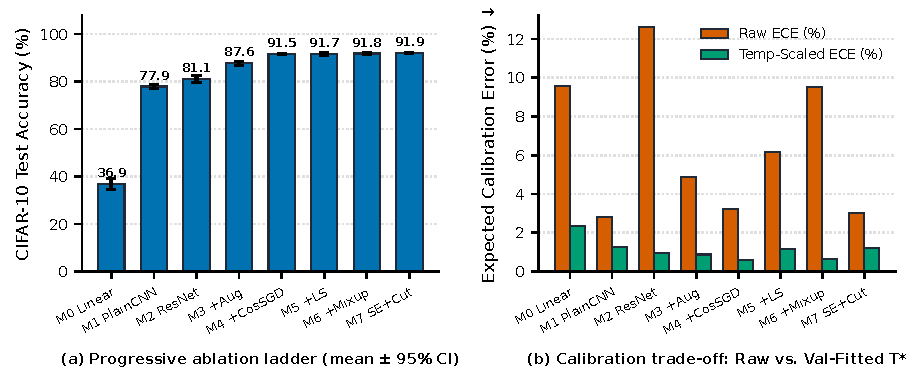
\includegraphics[width=\textwidth]{figures/fig_cifar10_ablation_and_ece.pdf}
  \caption{\textbf{CIFAR-10 progressive recipe ladder (24 RTX 3060 Ti runs, 30 epochs, 3 seeds) reveals strong accuracy gains alongside a non-monotonic calibration reversal.} (a) Held-out test accuracy (mean $\pm$ 95\% $t$-CI) climbs from \texttt{M0\_Linear} (\vlCMLinearTestAccMean{}) to \texttt{M7\_SEResNet\_Full} (\vlCMSeresnetFullTestAccMean{}). (b) Unaugmented \texttt{M2\_ResNet\_Base} exhibits severe overconfidence (raw ECE \vlCMResnetBaseTestEceMean{}), whereas Label Smoothing (\texttt{M5}) and Mixup (\texttt{M6}) induce underconfidence ($T^*<1$); strictly validation-fitted post-hoc Temperature Scaling reduces ECE across every residual arm.}
  \label{fig:c10_ablation}
\end{figure*}

\section{Results: Accuracy, Calibration, and Gate Trace}

\paragraph{CIFAR-10 progressive recipe gains (Table~\ref{tab:c10}, Figure~\ref{fig:c10_ablation}).}
Moving from \texttt{M1\_PlainCNN} (\vlCMPlaincnnTestAcc{}) to the deeper residual+BatchNorm \texttt{M2\_ResNet\_Base} (\vlCMResnetBaseTestAcc{}) improves CIFAR-10 held-out test accuracy across all three seeds, supporting \texttt{H1\_ResidualGain}.
Adding augmentation plus weight decay (\texttt{M3\_ResNet\_Aug}, \vlCMResnetAugTestAcc{}) and switching to warmup-cosine Nesterov SGD (\texttt{M4\_ResNet\_Aug\_Cosine}, \vlCMResnetAugCosineTestAcc{}) produce the largest bundled jumps, while \texttt{M7\_SEResNet\_Full} reaches \vlCMSeresnetFullTestAcc{} (95\% CI \vlCMSeresnetFullTestAccCi{}, delta +0.1406 / +14.06~pp over \texttt{M1\_PlainCNN}), supporting \texttt{H2\_AugCosineGain}.
By contrast, the modest accuracy differences of \texttt{M5\_ResNet\_LS} (+0.0021) and \texttt{M6\_ResNet\_Mixup} (\vlCMResnetMixupTestAcc{}) over \texttt{M4} lie within 3-seed CI overlap.

\begin{table*}[t]
\centering
\caption{\textbf{CIFAR-10 multi-seed held-out test results (30 epochs, 3 seeds, 24 GPU runs) auto-bound from TensorBoard and W\&B logs.} Every cell (including Mean $T^*$) is injected via \texttt{paper\_bind.py} macros; $T^*$ is fit strictly on validation logits.}
\label{tab:c10}
\setlength{\tabcolsep}{3.6pt}
\footnotesize
\resizebox{\textwidth}{!}{%
\begin{tabular}{lccccccc}
\toprule
\textbf{Method} & \textbf{Val Acc} & \textbf{Test Acc} & \textbf{Raw ECE $\downarrow$} & \textbf{Cal ECE $\downarrow$} & \textbf{Raw NLL $\downarrow$} & \textbf{Cal NLL $\downarrow$} & \textbf{Mean $T^*$} \\
\midrule
\texttt{M0\_Linear}            & \vlCMLinearValAcc{}          & \vlCMLinearTestAcc{}          & \vlCMLinearTestEce{}          & \vlCMLinearCalEce{}          & \vlCMLinearTestNll{}          & \vlCMLinearCalNll{}          & \vlCMLinearTempTMean{} \\
\texttt{M1\_PlainCNN}          & \vlCMPlaincnnValAcc{}        & \vlCMPlaincnnTestAcc{}        & \vlCMPlaincnnTestEce{}        & \vlCMPlaincnnCalEce{}        & \vlCMPlaincnnTestNll{}        & \vlCMPlaincnnCalNll{}        & \vlCMPlaincnnTempTMean{} \\
\texttt{M2\_ResNet\_Base}      & \vlCMResnetBaseValAcc{}      & \vlCMResnetBaseTestAcc{}      & \vlCMResnetBaseTestEce{}      & \vlCMResnetBaseCalEce{}      & \vlCMResnetBaseTestNll{}      & \vlCMResnetBaseCalNll{}      & \vlCMResnetBaseTempTMean{} \\
\texttt{M3\_ResNet\_Aug}       & \vlCMResnetAugValAcc{}       & \vlCMResnetAugTestAcc{}       & \vlCMResnetAugTestEce{}       & \vlCMResnetAugCalEce{}       & \vlCMResnetAugTestNll{}       & \vlCMResnetAugCalNll{}       & \vlCMResnetAugTempTMean{} \\
\texttt{M4\_ResNet\_Aug\_Cosine} & \vlCMResnetAugCosineValAcc{} & \vlCMResnetAugCosineTestAcc{} & \vlCMResnetAugCosineTestEce{} & \textbf{\vlCMResnetAugCosineCalEce{}} & \vlCMResnetAugCosineTestNll{} & \textbf{\vlCMResnetAugCosineCalNll{}} & \vlCMResnetAugCosineTempTMean{} \\
\texttt{M5\_ResNet\_LS}        & \vlCMResnetLsValAcc{}        & \vlCMResnetLsTestAcc{}        & \vlCMResnetLsTestEce{}        & \vlCMResnetLsCalEce{}        & \vlCMResnetLsTestNll{}        & \vlCMResnetLsCalNll{}        & \vlCMResnetLsTempTMean{} \\
\texttt{M6\_ResNet\_Mixup}     & \vlCMResnetMixupValAcc{}     & \vlCMResnetMixupTestAcc{}     & \vlCMResnetMixupTestEce{}     & \vlCMResnetMixupCalEce{}     & \vlCMResnetMixupTestNll{}     & \vlCMResnetMixupCalNll{}     & \vlCMResnetMixupTempTMean{} \\
\texttt{M7\_SEResNet\_Full}    & \textbf{\vlCMSeresnetFullValAcc{}} & \textbf{\vlCMSeresnetFullTestAcc{}} & \vlCMSeresnetFullTestEce{} & \vlCMSeresnetFullCalEce{} & \textbf{\vlCMSeresnetFullTestNll{}} & \vlCMSeresnetFullCalNll{} & \vlCMSeresnetFullTempTMean{} \\
\bottomrule
\end{tabular}}
\end{table*}

\paragraph{Calibration reversal under Label Smoothing and Mixup.}
Consistent with \citet{guo2017calibration}, unaugmented \texttt{M2\_ResNet\_Base} suffers severe overconfidence on CIFAR-10 (raw ECE \vlCMResnetBaseTestEce{}, raw NLL \vlCMResnetBaseTestNll{}), which validation-fitted $T^*=\vlCMResnetBaseTempTMean{}$ reduces to calibrated ECE \vlCMResnetBaseCalEce{} and calibrated NLL \vlCMResnetBaseCalNll{}.
Similarly, \texttt{M4\_ResNet\_Aug\_Cosine} drops from raw ECE \vlCMResnetAugCosineTestEce{} to \vlCMResnetAugCosineCalEce{} ($T^*=\vlCMResnetAugCosineTempTMean{}$), achieving both the lowest calibrated ECE and lowest calibrated NLL (\vlCMResnetAugCosineCalNll{}) across all eight CIFAR-10 arms.
Training-time target softening inverts the direction of miscalibration: \texttt{M5\_ResNet\_LS} raises raw ECE by +0.0295 to \vlCMResnetLsTestEce{} ($T^*=\vlCMResnetLsTempTMean{} < 1$, underconfident), and \texttt{M6\_ResNet\_Mixup} (tested on CIFAR-10 only) reaches raw ECE \vlCMResnetMixupTestEce{} ($T^*=\vlCMResnetMixupTempTMean{}$).
Sharpening logits with validation-fitted $T^*<1$ recovers calibrated ECE to \vlCMResnetLsCalEce{} (delta $-0.0503$) for \texttt{M5} and \vlCMResnetMixupCalEce{} for \texttt{M6}, confirming \texttt{H3\_CalibrationTradeoff}.

\begin{figure*}[t]
  \centering
  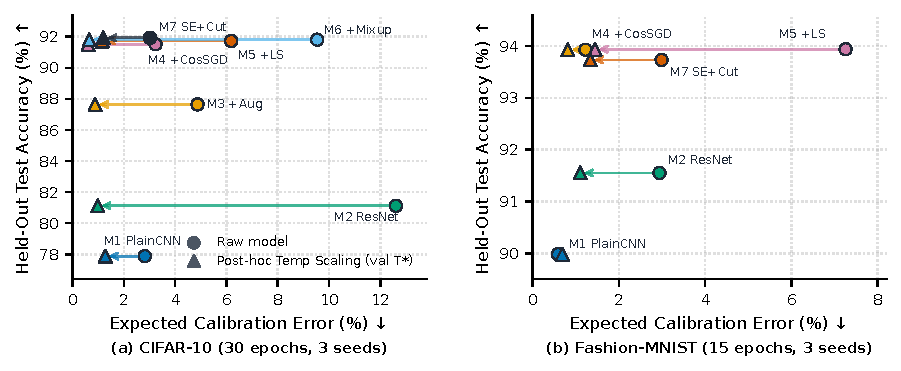
\includegraphics[width=\textwidth]{figures/fig_acc_ece_pareto.pdf}
  \caption{\textbf{Cross-dataset Accuracy--ECE Pareto frontier across CIFAR-10 (24 runs) and Fashion-MNIST (18 runs).} Circles show raw held-out test models and triangles show post-hoc validation-fitted Temperature Scaling ($T^*$); arrows trace the exact calibration shift for each method.}
  \label{fig:pareto}
\end{figure*}

\paragraph{Cross-dataset validation and honest nuance on Fashion-MNIST (Table~\ref{tab:fmnist}, Figure~\ref{fig:pareto}).}
On Fashion-MNIST (15 epochs, 18 runs; Mixup omitted), \texttt{M2\_ResNet\_Base} (\vlFMResnetBaseTestAcc{}) again outperforms \texttt{M1\_PlainCNN} (\vlFMPlaincnnTestAcc{}), and \texttt{M7\_SEResNet\_Full} (\vlFMSeresnetFullTestAcc{}) improves by +0.0375 (+3.75~pp) over \texttt{M1\_PlainCNN}, supporting \texttt{H4\_CrossDatasetRank}.
The Label Smoothing underconfidence reversal reproduces cleanly on Fashion-MNIST: \texttt{M5\_ResNet\_LS} lifts raw ECE by +0.0603 over \texttt{M4\_ResNet\_Aug\_Cosine} to \vlFMResnetLsTestEce{} ($T^*=\vlFMResnetLsTempTMean{}$), and validation-fitted $T^*$ reduces it by $-0.0581$ to \vlFMResnetLsCalEce{}.
Two honest nuances merit reporting without cherry-picking: (1) on already well-calibrated \texttt{M1\_PlainCNN} (raw ECE \vlFMPlaincnnTestEce{}, $T^*=\vlFMPlaincnnTempTMean{}$), post-hoc temperature scaling slightly increases test ECE to \vlFMPlaincnnCalEce{}; and (2) \texttt{M7\_SEResNet\_Full} (\vlFMSeresnetFullTestAcc{}) slightly trails \texttt{M4\_ResNet\_Aug\_Cosine} (\vlFMResnetAugCosineTestAcc{}) and \texttt{M5\_ResNet\_LS} (\vlFMResnetLsTestAcc{}), which we conjecture stems from $8\times 8$ Cutout occluding a larger fraction of $28\times 28$ grayscale garments than $32\times 32$ RGB scenes.

\begin{table*}[t]
\centering
\caption{\textbf{Fashion-MNIST cross-dataset results (15 epochs, 3 seeds, 18 GPU runs) auto-bound from TensorBoard and W\&B logs.} Every cell (including Mean $T^*$) is injected via \texttt{paper\_bind.py} macros.}
\label{tab:fmnist}
\setlength{\tabcolsep}{3.6pt}
\footnotesize
\resizebox{\textwidth}{!}{%
\begin{tabular}{lccccccc}
\toprule
\textbf{Method} & \textbf{Val Acc} & \textbf{Test Acc} & \textbf{Raw ECE $\downarrow$} & \textbf{Cal ECE $\downarrow$} & \textbf{Raw NLL $\downarrow$} & \textbf{Cal NLL $\downarrow$} & \textbf{Mean $T^*$} \\
\midrule
\texttt{M0\_Linear}            & \vlFMLinearValAcc{}          & \vlFMLinearTestAcc{}          & \vlFMLinearTestEce{}          & \vlFMLinearCalEce{}          & \vlFMLinearTestNll{}          & \vlFMLinearCalNll{}          & \vlFMLinearTempTMean{} \\
\texttt{M1\_PlainCNN}          & \vlFMPlaincnnValAcc{}        & \vlFMPlaincnnTestAcc{}        & \textbf{\vlFMPlaincnnTestEce{}} & \textbf{\vlFMPlaincnnCalEce{}} & \vlFMPlaincnnTestNll{}        & \vlFMPlaincnnCalNll{}        & \vlFMPlaincnnTempTMean{} \\
\texttt{M2\_ResNet\_Base}      & \vlFMResnetBaseValAcc{}      & \vlFMResnetBaseTestAcc{}      & \vlFMResnetBaseTestEce{}      & \vlFMResnetBaseCalEce{}      & \vlFMResnetBaseTestNll{}      & \vlFMResnetBaseCalNll{}      & \vlFMResnetBaseTempTMean{} \\
\texttt{M4\_ResNet\_Aug\_Cosine} & \vlFMResnetAugCosineValAcc{} & \vlFMResnetAugCosineTestAcc{} & \vlFMResnetAugCosineTestEce{} & \vlFMResnetAugCosineCalEce{} & \textbf{\vlFMResnetAugCosineTestNll{}} & \textbf{\vlFMResnetAugCosineCalNll{}} & \vlFMResnetAugCosineTempTMean{} \\
\texttt{M5\_ResNet\_LS}        & \textbf{\vlFMResnetLsValAcc{}} & \textbf{\vlFMResnetLsTestAcc{}} & \vlFMResnetLsTestEce{}        & \vlFMResnetLsCalEce{}        & \vlFMResnetLsTestNll{}        & \vlFMResnetLsCalNll{}        & \vlFMResnetLsTempTMean{} \\
\texttt{M7\_SEResNet\_Full}    & \vlFMSeresnetFullValAcc{}    & \vlFMSeresnetFullTestAcc{}    & \vlFMSeresnetFullTestEce{}    & \vlFMSeresnetFullCalEce{}    & \vlFMSeresnetFullTestNll{}    & \vlFMSeresnetFullCalNll{}    & \vlFMSeresnetFullTempTMean{} \\
\bottomrule
\end{tabular}}
\end{table*}

\begin{figure}[t]
  \centering
  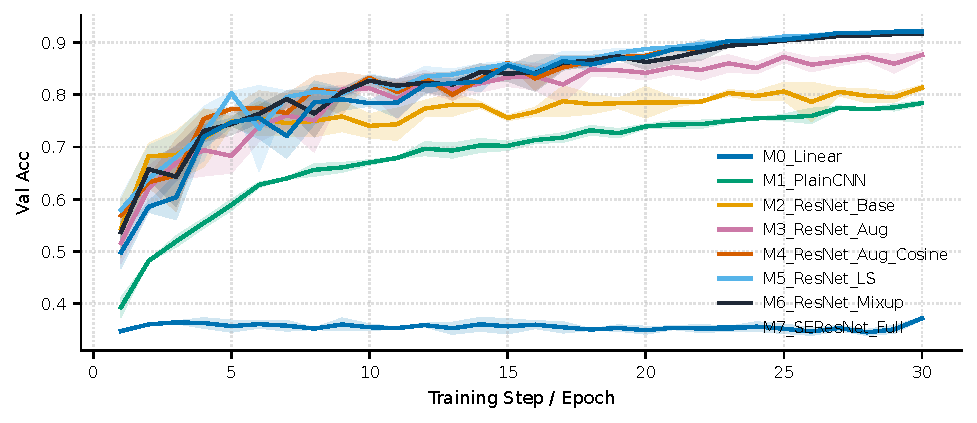
\includegraphics[width=\columnwidth]{bound/cifar10/bound_curves.pdf}
  \caption{\textbf{Validation accuracy trajectories automatically rendered by \texttt{./veriloop bind} directly from 72 CIFAR-10 TensorBoard and W\&B log files (mean $\pm$ std across 3 seeds).}}
  \label{fig:curves}
\end{figure}

\section{VeriLoop Governance Trace and Reproducibility}

Across the full 92.47~min RTX 3060 Ti run (5548.4~s total compute, 593.0~MB peak VRAM, PyTorch \texttt{2.9.1+cu128}), VeriLoop executed 14 automated stage self-consistency and AST smoke checks (8 CIFAR-10 stages + 6 Fashion-MNIST stages, Figure~\ref{fig:curves}): 14/14 passed (\texttt{passed=True}) on 182 distinct numbers in the final wiki re-audited across stages with 0 static-AST \texttt{HIGH} violations at 81.8~ms median gate latency and \$0 API cost.
Because the live wiki and \texttt{wiki\_metrics.log} are generated together from the same run summary, this stage gate verifies pipeline integrity and AST hygiene rather than serving as an independent tracing-recall test.
Independent end-to-end verification outputs are committed under \texttt{audits/}: \texttt{audits/claims\_check.txt} (4/4 claims passing 7/7 \texttt{G1--G7} gates with 0 revisions), \texttt{audits/veriloop\_gate.json} (\texttt{VERIFIABLE\_GATE: PASSED}), \texttt{audits/verify\_cites\_online.json} (10/10 arXiv/Crossref/S2 verified references), \texttt{audits/pdf\_audit.json} (expanded PDF numbers 100\% traced, 0 Type-3 fonts, 0 warnings), and the interactive split-pane \texttt{review\_ui.html}.

\bibliography{refs}
\bibliographystyle{icml2027}

\end{document}
